\documentclass[11pt]{article}
\usepackage[T1]{fontenc}
\usepackage[margin=1in]{geometry}
\usepackage{amsmath,amssymb,amsthm}
\usepackage{graphicx}
\usepackage[colorlinks=true,linkcolor=blue,citecolor=blue,urlcolor=blue]{hyperref}
\theoremstyle{remark}
\newtheorem{remark}{Remark}[section]
\newcommand{\Tr}{\operatorname{Tr}}
\newcommand{\deff}{d_{\rm eff}}

\title{Emergent Information Distance from Petz Recovery\\
{\large Temperature and perturbation dependence in TFIM exact
diagonalization}\\
{\normalsize Version 2}}
\author{Lluis Eriksson\\ Independent Researcher\\ \texttt{lluiseriksson@gmail.com}}
\date{January 2026 (v1); July 2026 (v2)}

\begin{document}
\maketitle

\begin{abstract}
We define an operational notion of effective distance from approximate
quantum state recovery. Given a tripartition $A$--$B$--$C$ with $B$ a
collar of width $w$ separating $A$ from $C$, we compute a Petz recovery
reconstruction error $E_{\rm Petz}(w) = -\log F(\rho_{ABC},
\tilde\rho^{\rm Petz}_{ABC}(w))$ (squared Uhlmann fidelity) and define an
emergent distance $\deff(\varepsilon)$ as the minimal collar width such
that the best-achieved error up to $w$ falls below a threshold
$\varepsilon$. Using exact diagonalization for the transverse-field Ising
chain at $N = 11$, $h_x = 1.05$, $|A| = 2$, we find that
$\deff(10^{-3})$ grows strongly with inverse temperature $\beta$ in the
unperturbed case ($h_z = 0$), from $1.00$ at $\beta = 0.5$ to $3.57$ at
$\beta = 5.0$, while remaining near-minimal in the longitudinally
perturbed case ($h_z = 0.5$), close to $1.0$ across the same range. We
also introduce a discrete curvature diagnostic based on second
differences of $\log E_{\rm Petz}(w)$ on a pre-floor window, reported
only when identifiable. \emph{v2 (no v1 number is changed):} the garbled
reproducibility paragraph of v1 is replaced by a real, regenerable
verification suite, which reproduces the $\beta$-sweep to two decimals
already at $N = 9$ ($\deff = 1.00, 1.00, 1.51, 2.11, 2.82, 3.55$ vs
$3.57$ at $N = 11$; $\mu_{\rm prefloor}$ endpoints $8.44 \to 1.35$ vs
$1.33$; PSD-projection sensitivity $3.3\times10^{-8}$ vs
$\sim 3\times10^{-8}$) -- independently confirming the finite-size
robustness of the appendix; the mild $|C|$-shrinkage caveat is stated
with cross-references to its quantified analysis in the companions; and
series positioning is added.
\end{abstract}

\section{Introduction}
Motivated by the theme that locality and entanglement structure constrain
information flow, we extract a geometry-like diagnostic directly from
approximate recoverability: recovery performance is the primitive
observable, and an effective distance is the minimal separation needed to
reach a fixed recovery-error threshold. Scope: we do not attempt to
derive gravitational field equations; the goal is a minimal, falsifiable
construction of an emergent geometric \emph{diagnostic} -- an operational
quantity depending on the threshold, temperature, protocol and geometry,
not a universal length.

\paragraph{Series positioning (added in v2).} This note completes the
$\deff$ mini-block of the recovery program: 2601.0038 \cite{S0038}
introduced $\deff$ and its criticality signature in $h_x$; 2601.0040
\cite{S0040} studied its finite-size scaling (whose $|C|$/baseline and
functional-form caveats apply mutatis mutandis here); the present note
fixes $h_x = 1.05$ and varies $(\beta, h_z)$. The ED/Petz pipeline and
censored-reporting discipline are those of 2601.0035 \cite{S0035}, with
the non-Gaussian bridge upstream in 2512.0101 \cite{S0101}.

\section{Setup and definitions}
As in the companions: $E_{\rm Petz}(w) := -\log F(\rho_{ABC},
\tilde\rho^{\rm Petz}_{ABC}(w))$, $F(\rho,\sigma) =
(\Tr\sqrt{\sqrt\rho\,\sigma\sqrt\rho})^2$;
$\mathcal{R}^{\rm Petz}_{B\to BC}(X_B) = \rho_{BC}^{1/2}\rho_B^{-1/2}
X_B \rho_B^{-1/2}\rho_{BC}^{1/2}$ with spectral floor
$\lambda_{\min} = 10^{-12}$ applied only in $\rho_B^{-1/2}$;
hermitization, PSD projection and trace renormalization applied to the
output (direct check: this post-processing changes $E_{\rm Petz}$ by at
most $\sim 3\times10^{-8}$; the suite reproduces $3.3\times10^{-8}$);
$E_{\rm best}(w) := \min_{w' \le w} E_{\rm Petz}(w')$;
$\deff(\varepsilon) := \min\{w : E_{\rm best}(w) \le \varepsilon\}$ with
log-linear interpolation. Pre-floor window $E_{\rm Petz}(w) \ge
10\,y_{\min}$ with $y_{\min} = 10^{-12}$ (distinct from
$\lambda_{\min}$); discrete curvature $\kappa(w)$ by second differences
of $\log E_{\rm Petz}$, summarized by $\bar\kappa$ only when at least
three consecutive widths are pre-floor.

\begin{remark}[$|C|$ caveat (added in v2)]
Here $w \le 5$ at $N = 11$, so $|C| \ge 4$ and the $|C|$-shrinkage
confound quantified in 2601.0038/0040 v2 is mild; nevertheless, absolute
$\deff$ values inherit the tripartition geometry, and all claims below
are regime \emph{comparisons} at fixed geometry ($h_z = 0$ vs $0.5$ at
the same $(N, |A|, w)$), which are unaffected.
\end{remark}

\section{Data and methodology}
As in v1: $H = -J\sum Z_iZ_{i+1} - h_x\sum X_i - h_z\sum Z_i$, open
boundaries, $J = 1$, $h_x = 1.05$, $h_z \in \{0, 0.5\}$; Gibbs states by
ED; $A = \{1,2\}$, $B = \{3,\dots,2{+}w\}$, $C$ the rest; $w \in
\{1,\dots,5\}$ at $N = 11$; pre-floor fits $\log E_{\rm Petz}(w) \approx
a - \mu_{\rm prefloor} w$ with identifiability reported via
$(n_{\rm prefloor}, n_\kappa)$.

\section{Results}
All v1 numbers stand.
\textbf{Effective distance vs temperature:} at $\varepsilon = 10^{-3}$,
$\deff = 1.00, 1.00, 1.51, 2.11, 2.82, 3.57$ for $h_z = 0$ and
$1.00, 1.00, 1.00, 1.00, 1.02, 1.04$ for $h_z = 0.5$ ($\beta = 0.5,
\dots, 5$); Figures~\ref{fig:profiles}--\ref{fig:sens}.
\textbf{Threshold sensitivity:} the regime ordering
$\deff|_{h_z=0} \ge \deff|_{h_z=0.5}$ holds for $\varepsilon \in
\{10^{-2}, 10^{-3}, 10^{-4}\}$ across all sampled $\beta$.
\textbf{Decay proxy and curvature:} $\mu_{\rm prefloor}$ falls from
$\approx 8.44$ ($\beta = 0.5$) to $\approx 1.33$ ($\beta = 5$) at
$h_z = 0$ while staying in $\approx [4.16, 8.56]$ at $h_z = 0.5$;
$\bar\kappa$ is identifiable only at $h_z = 0$, $\beta \ge 1$
($(n_{\rm prefloor}, n_\kappa) \in \{(3,1), (5,3)\}$; e.g.\ $\bar\kappa
\approx 1.97$ at $\beta = 1$, $0.44$ at $\beta = 3$), and undefined at
$h_z = 0.5$ ($n_{\rm prefloor} = 2$) -- by policy, reported as ``---''.

\begin{figure}[h]\centering
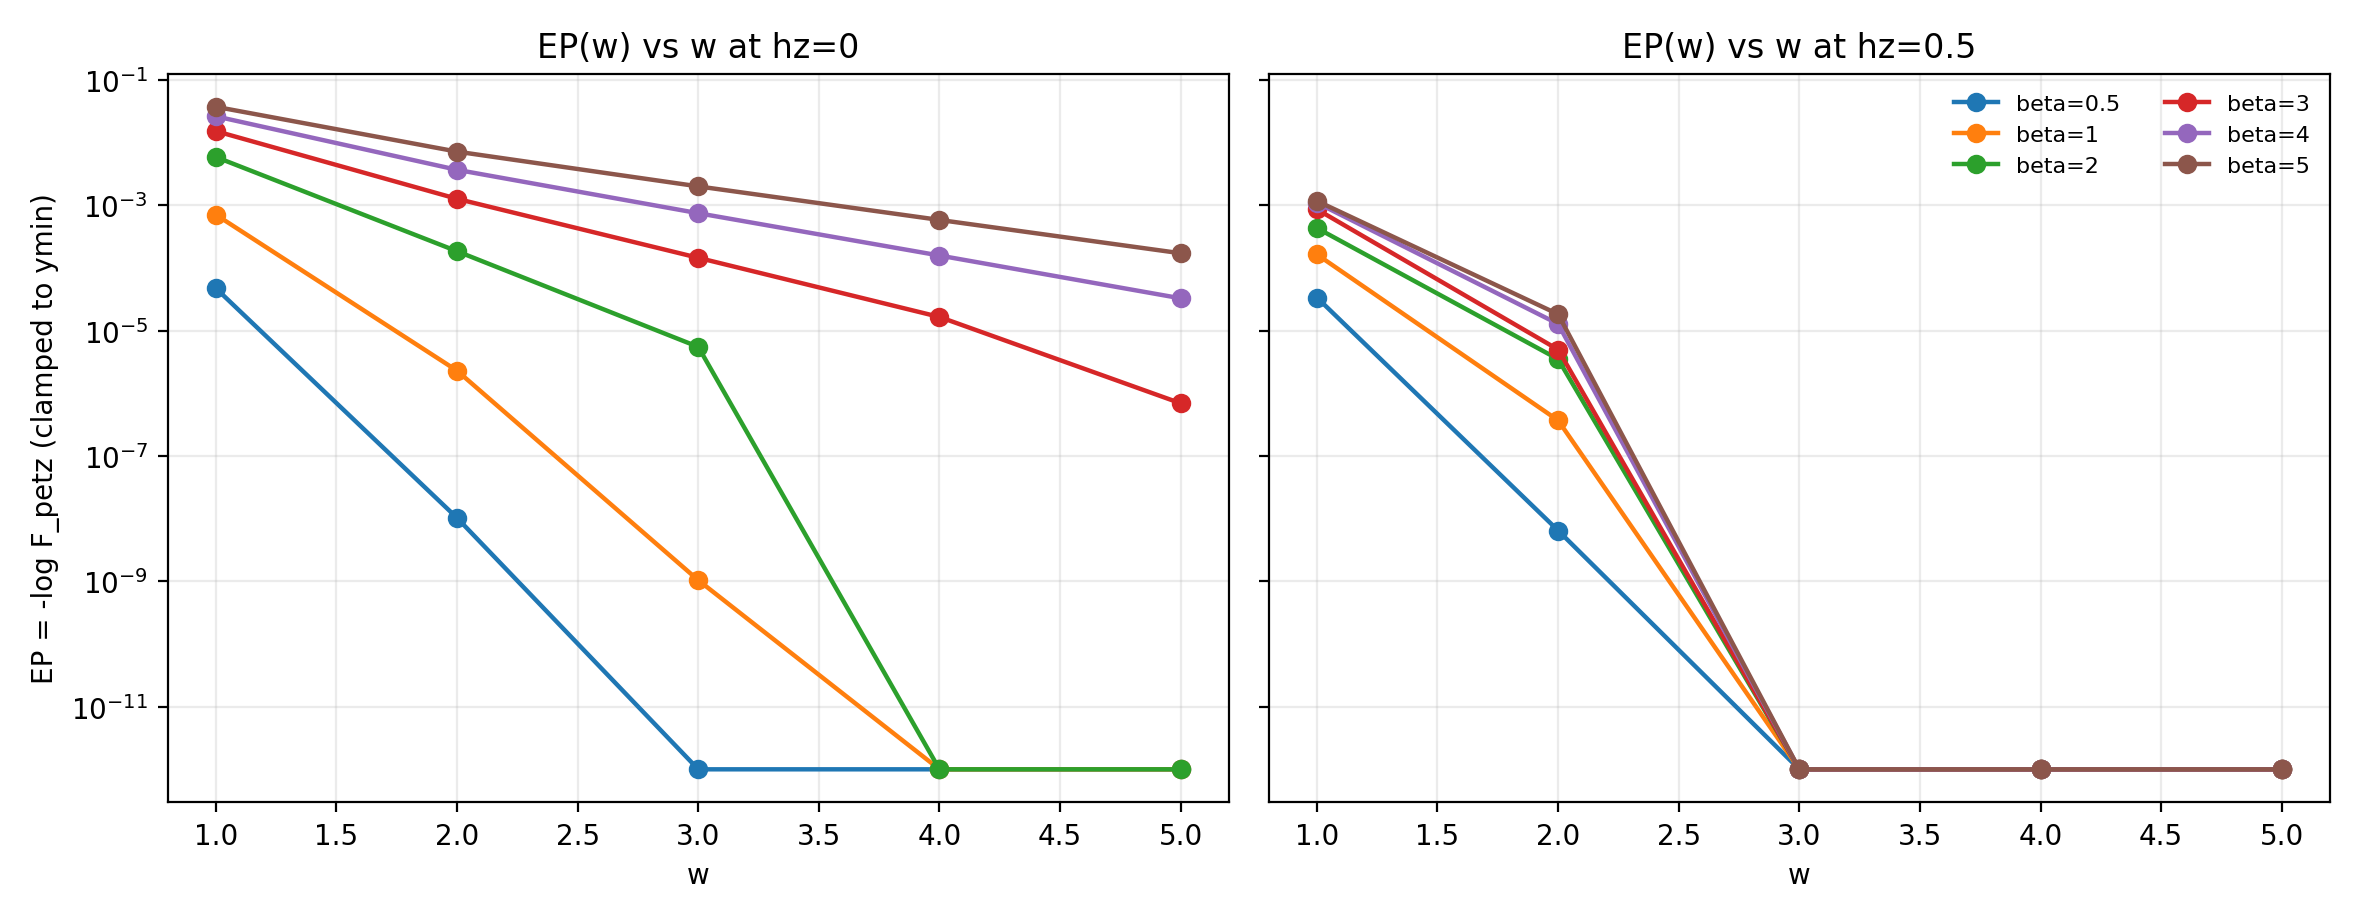
\includegraphics[width=0.95\textwidth]{fig1_profiles.png}
\caption{$E_{\rm Petz}(w)$ vs $w$ (log scale, clamped at $y_{\min} =
10^{-12}$). Left: $h_z = 0$; right: $h_z = 0.5$ (v1 figure, unchanged).}
\label{fig:profiles}
\end{figure}
\begin{figure}[h]\centering
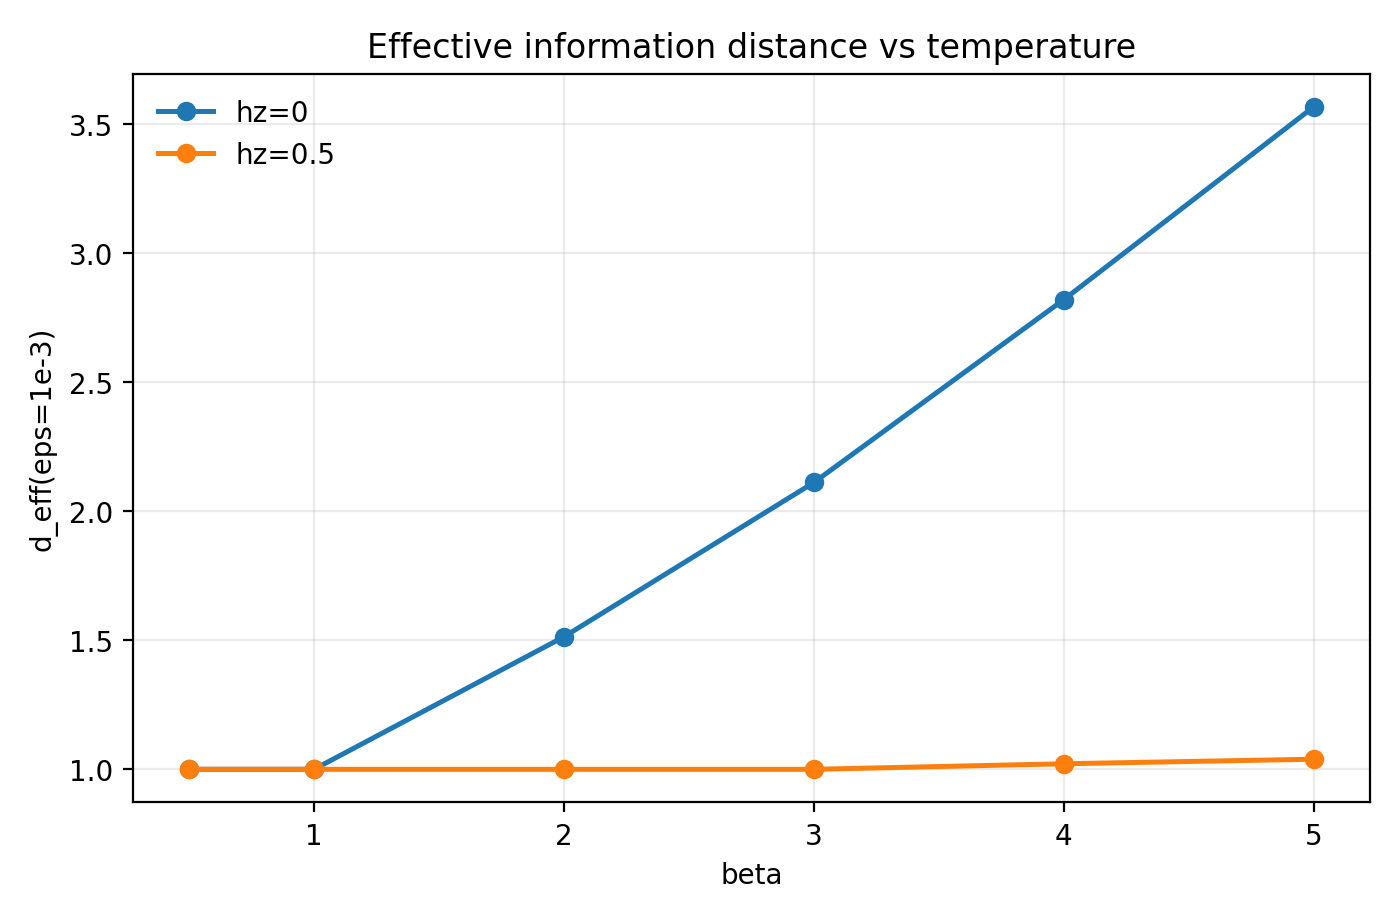
\includegraphics[width=0.62\textwidth]{fig2_deff_beta.png}
\caption{$\deff(10^{-3})$ vs $\beta$ for both regimes (v1 figure,
unchanged).}
\label{fig:deff}
\end{figure}
\begin{figure}[h]\centering
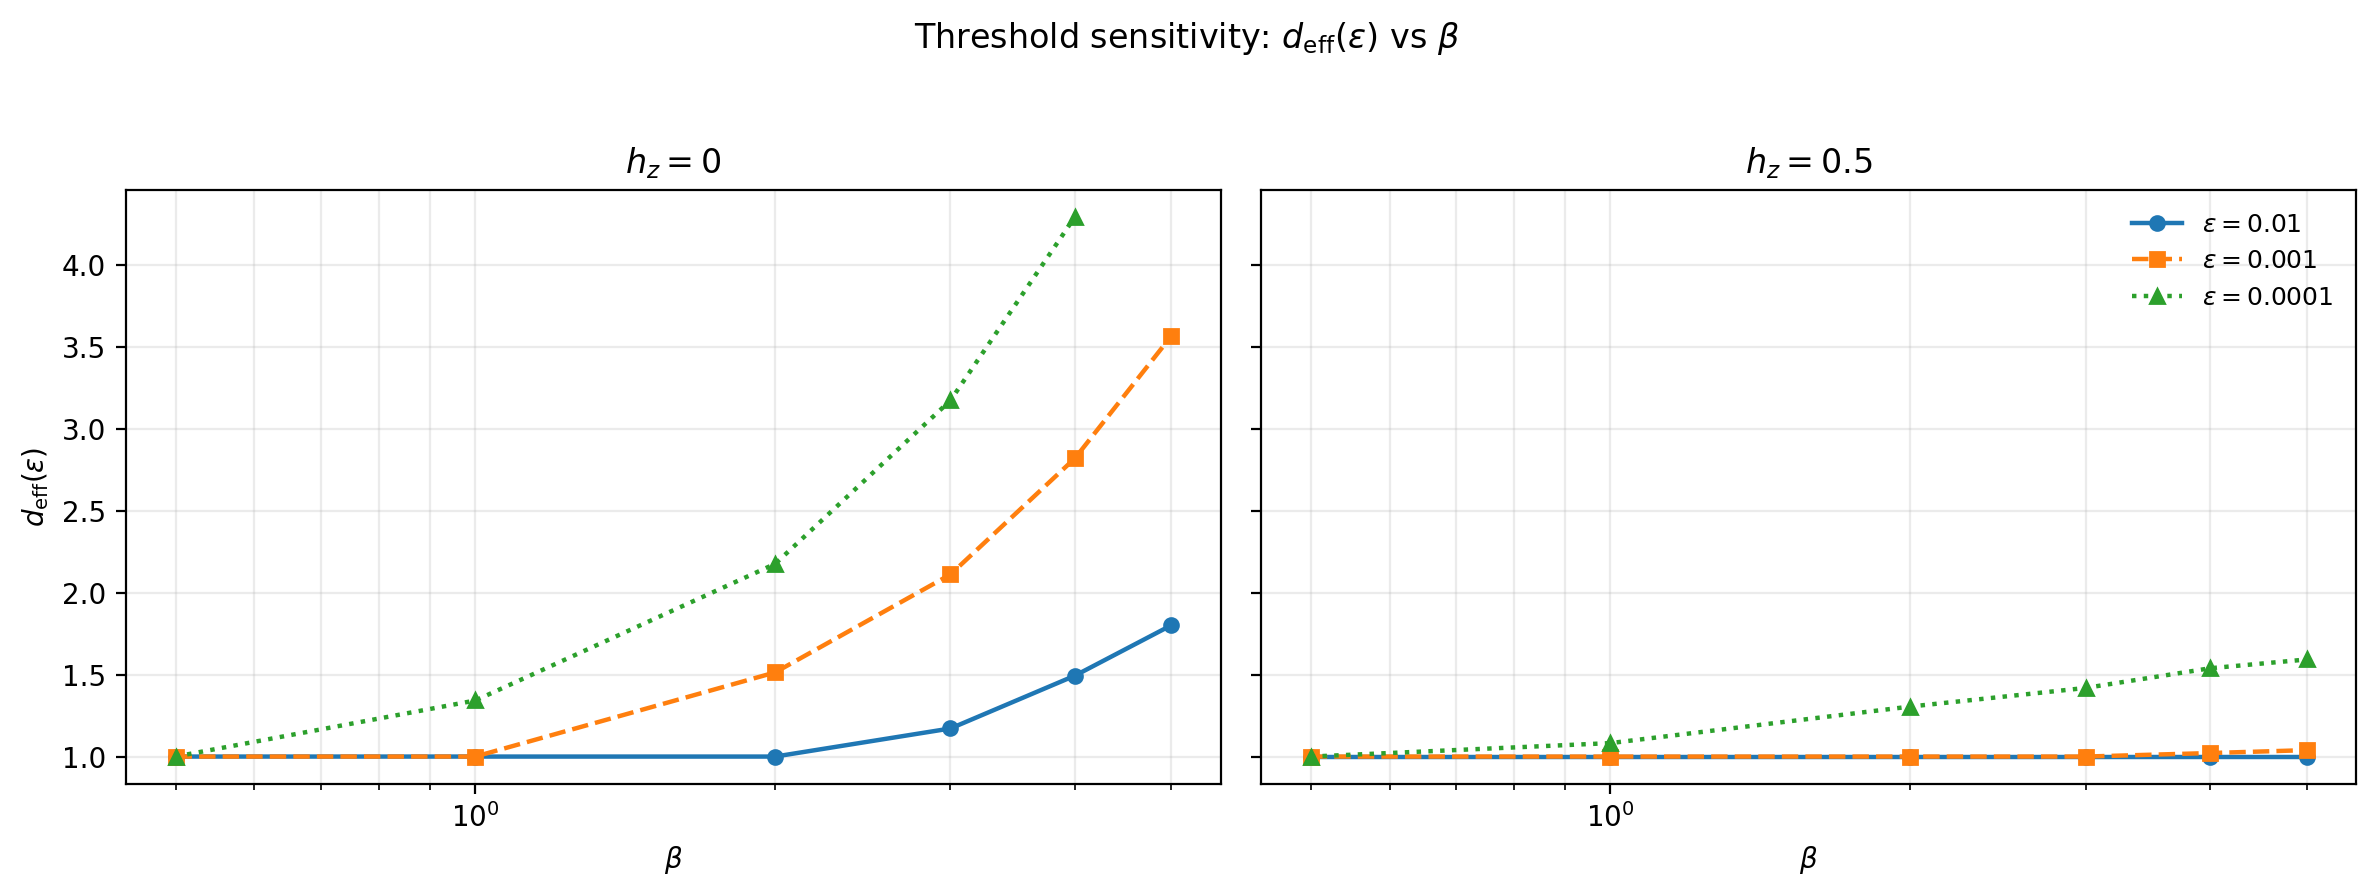
\includegraphics[width=0.8\textwidth]{fig3_threshold.png}
\caption{Threshold sensitivity: $\deff(\varepsilon)$ vs $\beta$,
$\varepsilon \in \{10^{-2}, 10^{-3}, 10^{-4}\}$ (v1 figure, unchanged).}
\label{fig:sens}
\end{figure}

\section{Verification suite (rewritten in v2)}
v1's reproducibility paragraph was corrupted in production (a garbled
reference to a patched driver \texttt{run\_edp\_sdproj.py}) and referred
vaguely to CSV artifacts ``possibly included'' in an Overleaf bundle. v2
replaces it: \texttt{verification/2601-0042/verify\_2601\_0042.py}
(regenerable ED, chunked JSON cache, default $N = 9$, \texttt{--N11} for
the paper size) recomputes the entire pipeline from scratch and checks:
the $\beta$-growth of $\deff$ at $h_z = 0$ and near-minimality at
$h_z = 0.5$ (reproducing the v1 values to two decimals already at
$N = 9$); the regime ordering across all three thresholds; the decrease
of $\mu_{\rm prefloor}$ with $\beta$; the $\bar\kappa$ identifiability
policy; and the PSD-projection sensitivity bound. The close $N = 9$ vs
$N = 11$ agreement independently confirms the finite-size robustness
check of the appendix ($N = 11$ vs $12$).

\section{Limitations and outlook}
As in v1, sharpened: $\deff$ is an operational diagnostic -- threshold-,
temperature-, protocol- and geometry-dependent -- not a universal
correlation length; the connection of its $\beta$-growth at $h_x = 1.05$
to the near-critical ground state (and its suppression by a
symmetry-breaking $h_z$) is physically natural and consistent with the
$h_x$-signature of 2601.0038, but establishing scaling requires the
fixed-$|C|$ protocols and larger sizes discussed in 2601.0040 v2.
Comparing to CMI-based diagnostics (cf.\ 2601.0038 v2) is a natural next
step.

\appendix
\section{Finite-size robustness (v1 figure, unchanged)}
\begin{figure}[h]\centering
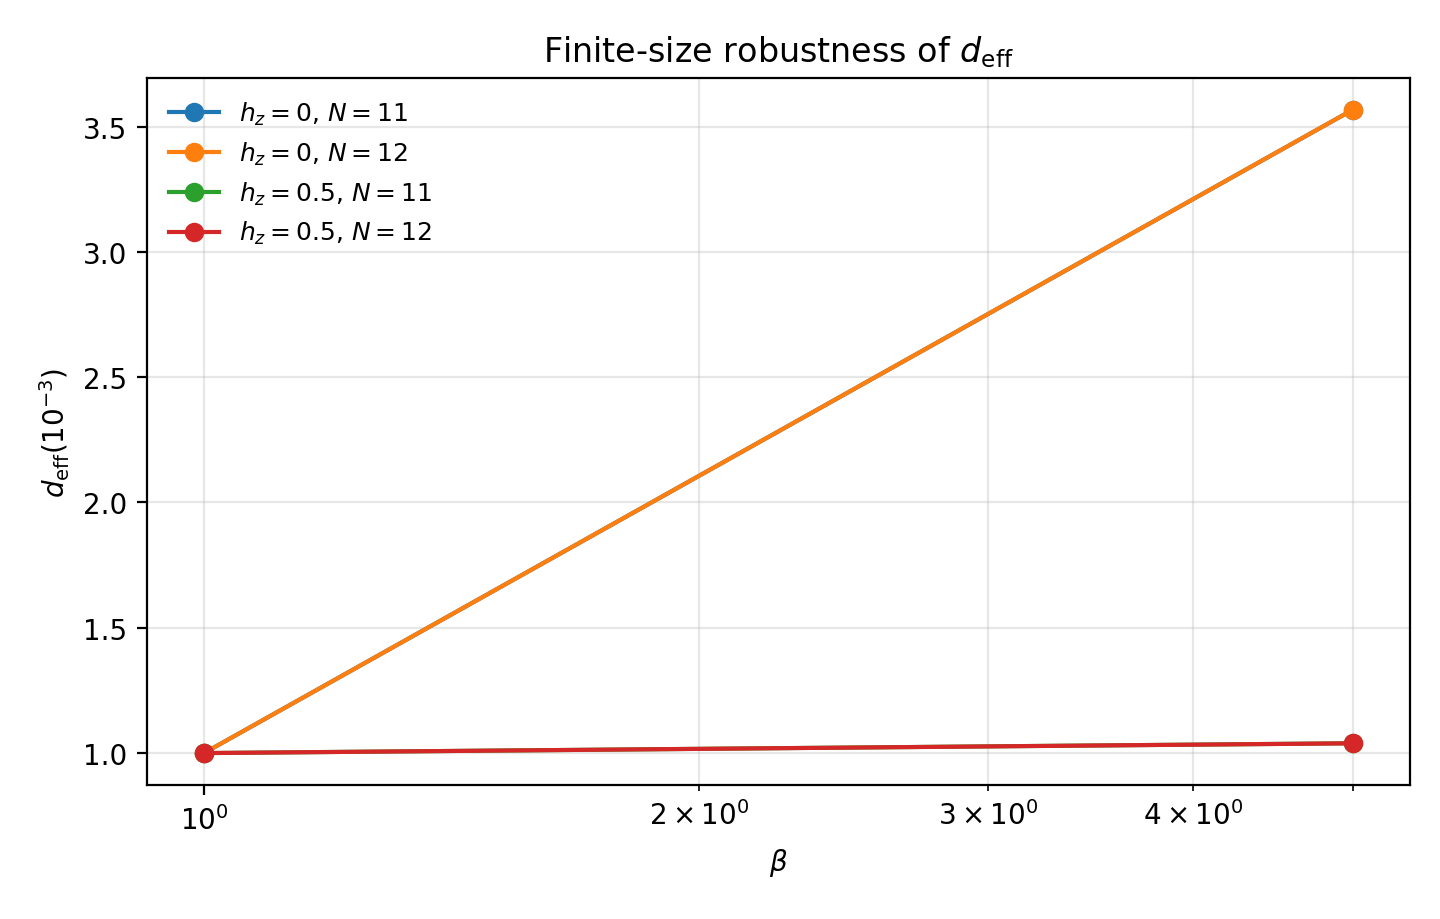
\includegraphics[width=0.6\textwidth]{fig4_sizecheck.png}
\caption{$N = 11$ vs $N = 12$ robustness check from v1; independently
corroborated by the $N = 9$ reproduction of the suite.}
\end{figure}

\section*{Note added in v2}
No v1 number is changed; all figures, tables and the appendix stand, and
the suite reproduces the headline numbers to two decimals at $N = 9$.
Changes: (1) the corrupted reproducibility paragraph of v1 is replaced by
a real verification suite; (2) the mild $|C|$ caveat is stated with
cross-references to its quantified analysis in 2601.0038/0040 v2; (3)
series positioning added (v1 cited no companion papers despite sharing
definitions verbatim with 2601.0038); (4) the ``emergent distance''
reading is explicitly framed as an operational diagnostic.

\begin{thebibliography}{8}
\bibitem{FR} O. Fawzi and R. Renner, Commun. Math. Phys. \textbf{340}
(2015) 575--611.
\bibitem{JRSWW} M. Junge et al., Ann. Henri Poincar\'e \textbf{19} (2018)
2955--2978.
\bibitem{Petz} D. Petz, Commun. Math. Phys. \textbf{105} (1986)
123--131.
\bibitem{Sachdev} S. Sachdev, \emph{Quantum Phase Transitions}, 2nd ed.,
Cambridge University Press (2011).
\bibitem{S0038} L. Eriksson, ai.viXra:2601.0038 (2026; v2 2026).
\bibitem{S0040} L. Eriksson, ai.viXra:2601.0040 (2026; v2 2026).
\bibitem{S0035} L. Eriksson, ai.viXra:2601.0035 (2026; v2 2026).
\bibitem{S0101} L. Eriksson, ai.viXra:2512.0101 (2025; v2 2026).
\end{thebibliography}
\end{document}
